\section{实验与结果}

\subsection{实验设置}

硬件为 RTX 4060 Laptop（8 GB），PyTorch 2.15。除非特别说明，模型均为 RGB 基线、580 个训练身份、3,600 帧测试集。训练曲线见图~\ref{fig:train}。

\begin{figure}[H]
\centering
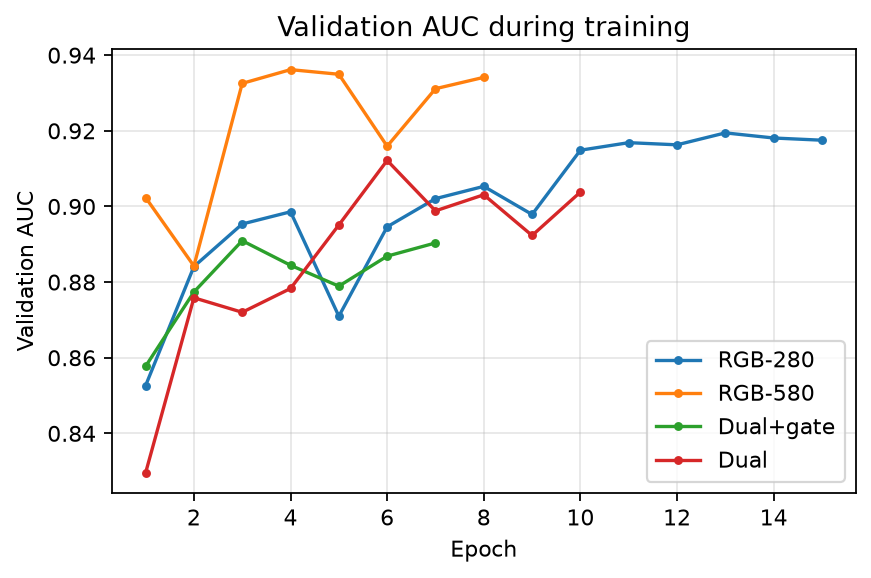
\includegraphics[width=0.72\linewidth]{fig_training_curve.png}
\caption{各模型验证集 AUC 随训练轮次的变化}
\label{fig:train}
\end{figure}

\subsection{同库结果}

\begin{table}[H]
\centering
\caption{同库结果（测试集 3,600 帧 / 180 条视频）}
\label{tab:indomain}
\scriptsize
\setlength{\tabcolsep}{3.5pt}
\begin{tabular}{lcccccc}
\toprule
\multirow{2}{*}{模型} & \multicolumn{2}{c}{帧级} & \multicolumn{2}{c}{视频级} & \multirow{2}{*}{F1@0.5} & \multirow{2}{*}{FPR@0.5} \\
\cmidrule(lr){2-3}\cmidrule(lr){4-5}
 & AUC & TPR@1\% & AUC & TPR@1\% & & \\
\midrule
E1 RGB-8ep & 0.8763 & 0.231 & -- & -- & 0.850 & 24.0\% \\
E2 RGB-280 & 0.9115 & 0.365 & 0.9308 & 0.425 & 0.870 & 16.6\% \\
\textbf{E9 RGB-580} & \textbf{0.9328} & \textbf{0.596} & \textbf{0.9499} & \textbf{0.700} & \textbf{0.886} & 10.5\% \\
\bottomrule
\end{tabular}
\end{table}

E1 暴露了两个问题：训练时 100\% 加退化、测试是干净图，分布不匹配；且按 F1@FPR1\% 选模型噪声大。E2 把退化概率降到 50\%、改按 AUC 选模型、加类别权重，AUC 提升 0.057。E9 把训练身份从 280 扩到 580，AUC 再提升 0.021，低误报召回提升 23 个百分点，说明数据量是此前的瓶颈之一。

\subsection{双流与门控消融}

\begin{table}[H]
\centering
\caption{双流与门控消融}
\label{tab:ablation}
\small
\begin{tabular}{lccc}
\toprule
模型 & 帧级 AUC & 视频级 AUC & 跨库 AUC \\
\midrule
RGB（E2） & 0.9115 & 0.9308 & 0.6687 \\
双流 + 门控（E3） & 0.9088 & \textbf{0.9411} & 0.6666 \\
双流无门控（E3b） & 0.9067 & 0.9297 & 0.6823 \\
\bottomrule
\end{tabular}
\end{table}

三者差异在 $\pm 0.011$ 内且互有胜负，属于划分与随机种子噪声。\textbf{频域分支未带来稳定收益。}

\textbf{门控失效分析}：在 1,408 张测试图上统计，门控输出均值 0.4272、标准差 \textbf{0.0008}，真图 0.4274、假图 0.4271，几乎是一个常数（图~\ref{fig:gate}）。原因有两层：其一，门控输入 $\log(1+10h_f)$ 中 $h_f$ 仅约 0.005，输入变化范围不足 0.01；其二，真假图的高频能量分布几乎完全重叠（真 $0.0053\pm0.0010$，假 $0.0049$--$0.0058$），该“质量代理”本身没有区分度。因此门控不是“没训好”，而是设计前提不成立。

\begin{figure}[H]
\centering
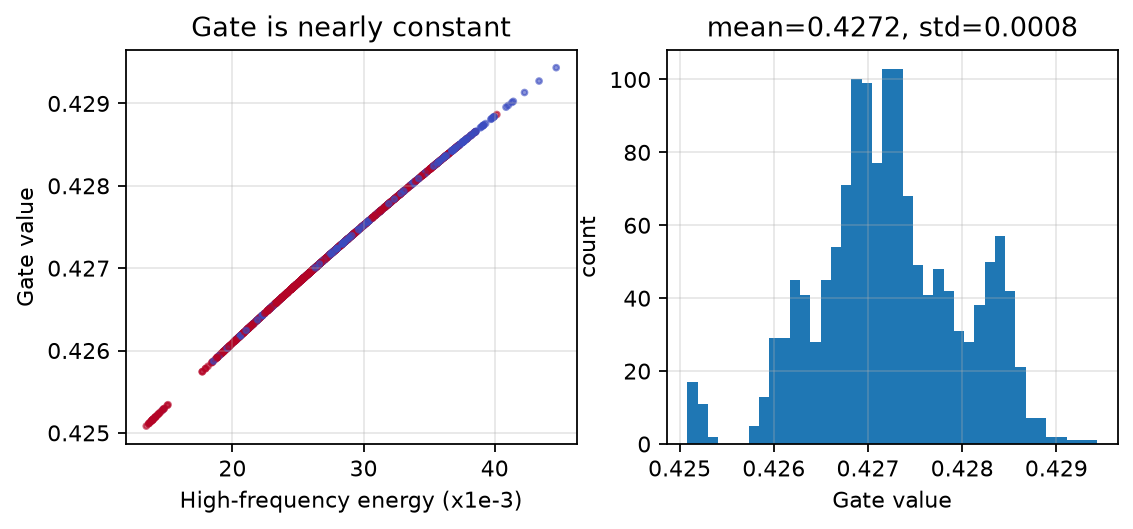
\includegraphics[width=0.9\linewidth]{fig_gate.png}
\caption{门控值随高频能量的变化（左）与分布（右）：几乎恒为 0.427}
\label{fig:gate}
\end{figure}

\textbf{频谱分析}：对 200 张真图与 200 张假图求平均 log 幅度谱并相减，差异集中在水平与垂直两条轴上，呈明显十字形（图~\ref{fig:specdiff}），其余区域接近噪声。轴对齐的强差异更符合 JPEG $8\times8$ 块效应与重采样的形态，而非生成器指纹。这解释了频域分支为何同库不涨、跨库不迁移。

\begin{figure}[H]
\centering
\begin{subfigure}{0.31\linewidth}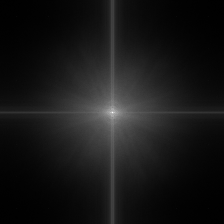
\includegraphics[width=\linewidth]{spectrum_real.png}\caption{真图平均谱}\end{subfigure}
\hfill
\begin{subfigure}{0.31\linewidth}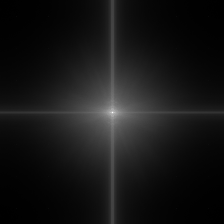
\includegraphics[width=\linewidth]{spectrum_fake.png}\caption{假图平均谱}\end{subfigure}
\hfill
\begin{subfigure}{0.31\linewidth}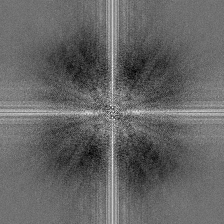
\includegraphics[width=\linewidth]{spectrum_diff.png}\caption{差异（假$-$真）}\end{subfigure}
\caption{真假平均频谱与差异：差异呈轴对齐十字形，更像压缩块效应}
\label{fig:specdiff}
\end{figure}

\subsection{鲁棒性矩阵}

\begin{table}[H]
\centering
\caption{主模型（RGB-580）在不同退化下的表现（冻结阈值）}
\label{tab:robust}
\small
\begin{tabular}{lccccc}
\toprule
退化 & AUC & F1 & 召回 & FPR & TPR@1\% \\
\midrule
干净 & 0.9328 & 0.652 & 0.484 & 0.33\% & 0.596 \\
JPEG 70 & 0.9123 & 0.664 & 0.500 & 1.25\% & 0.493 \\
JPEG 50 & 0.8896 & 0.633 & 0.467 & 1.67\% & 0.394 \\
JPEG 30 & 0.8617 & 0.540 & 0.372 & 1.25\% & 0.363 \\
噪声 $\sigma=5$ & 0.8984 & 0.529 & 0.360 & 0.58\% & 0.484 \\
模糊 $5\times5$ & 0.8933 & 0.424 & 0.270 & 0.33\% & 0.353 \\
下采样 0.5 & 0.8988 & 0.471 & 0.309 & 0.67\% & 0.354 \\
裁剪 10\% & 0.9180 & 0.575 & 0.405 & 0.58\% & 0.471 \\
\bottomrule
\end{tabular}
\end{table}

\begin{figure}[H]
\centering
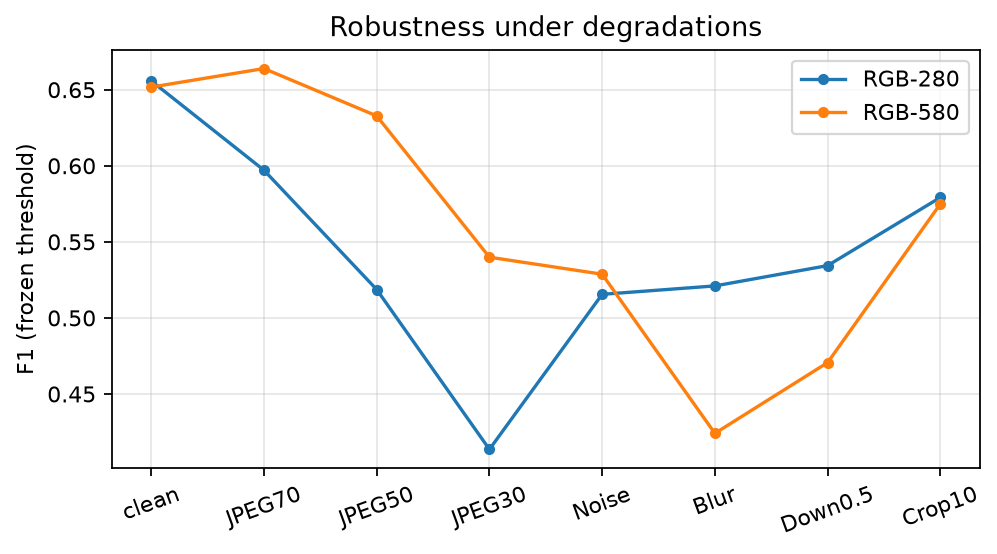
\includegraphics[width=0.78\linewidth]{fig_robustness.png}
\caption{两种训练规模下的鲁棒性曲线}
\label{fig:robust}
\end{figure}

与 280 身份版本相比，JPEG 鲁棒性明显改善（JPEG30 掉点从 24.2 pt 降到 11.2 pt），但模糊与下采样变差，说明模型仍依赖高频细节。TPR@1\% 在所有退化下都下降，表明排序能力本身受损，不只是阈值漂移。

\subsection{跨库结果}

\begin{table}[H]
\centering
\caption{跨库 Celeb-DF 结果（阈值冻结）}
\label{tab:cross}
\small
\begin{tabular}{lccc}
\toprule
模型 & 跨库 AUC & 跨库 TPR@1\% & 跨库 TPR@10\% \\
\midrule
E2（280 身份） & 0.6687 & 0.041 & -- \\
E9（580 身份） & \textbf{0.7163} & 0.068 & 0.281 \\
\bottomrule
\end{tabular}
\end{table}

扩数据让跨库 AUC 提升 0.048，说明更多身份带来了一点更通用的线索；但 0.716 仍不足以称为“跨库可用”，域偏移问题没有解决。冻结阈值下跨库 F1 很低，再次说明源域阈值不能直接迁移。图~\ref{fig:roc} 给出了主模型在同库与跨库上的 ROC 曲线。

\begin{figure}[H]
\centering
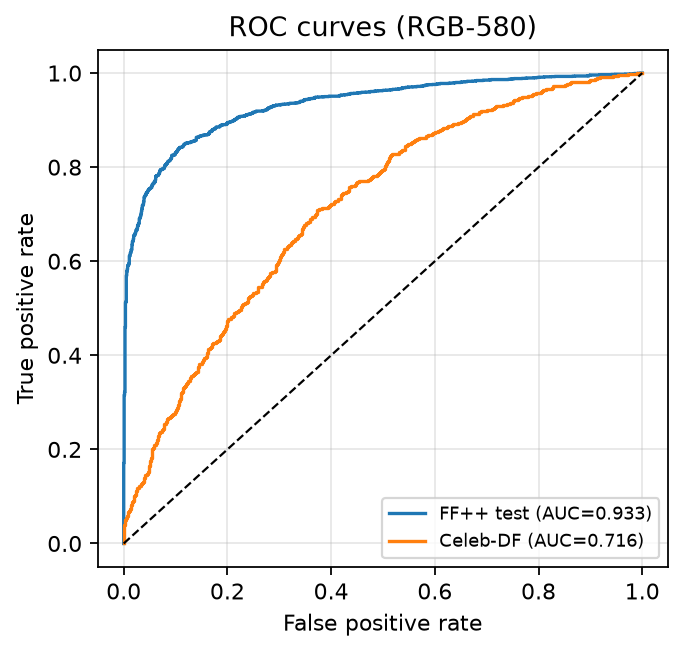
\includegraphics[width=0.55\linewidth]{fig_roc.png}
\caption{同库与跨库 ROC 曲线}
\label{fig:roc}
\end{figure}

\begin{figure}[H]
\centering
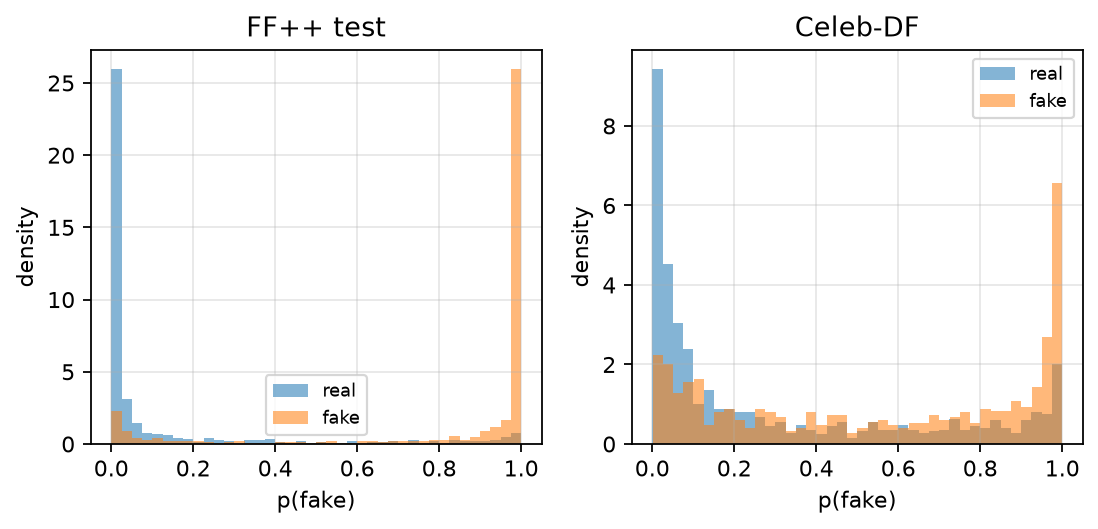
\includegraphics[width=0.85\linewidth]{fig_score_dist.png}
\caption{真、假样本的分数分布（左：FF++；右：Celeb-DF）}
\label{fig:dist}
\end{figure}

\subsection{未见伪造方法}

训练时完全移除 FaceShifter，测试集只含真人 + FaceShifter：

\begin{table}[H]
\centering
\caption{未见方法（FaceShifter）泛化}
\label{tab:unseen}
\small
\begin{tabular}{lccc}
\toprule
训练身份 & AUC & TPR@1\% & TPR@10\% \\
\midrule
280 & 0.5463 & 0.000 & 0.053 \\
580 & 0.5975 & 0.000 & 0.087 \\
\bottomrule
\end{tabular}
\end{table}

数据量翻倍只把 AUC 从 0.546 提到 0.598，1\% 误报下仍抓不到任何一张。对比同库 TPR@1\% 从 0.365 提到 0.596、跨库 AUC 从 0.669 提到 0.716，可见\textbf{扩数据改善“见过的类型”和“域内差异”，但解决不了“没见过的生成方法”}。后者是捷径学习问题。

\subsection{可解释性}

\textbf{Grad-CAM}：对 RGB 分支最后一层卷积做梯度加权，热图集中在眼、鼻、口区域（图~\ref{fig:cam}），定性合理。

\begin{figure}[H]
\centering
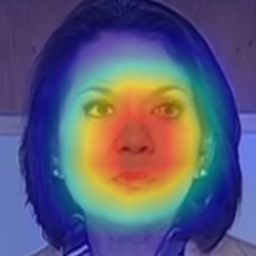
\includegraphics[width=0.34\linewidth]{heatmap_example.png}
\caption{Grad-CAM 热图示例}
\label{fig:cam}
\end{figure}

\textbf{定量 faithfulness}：取 100 张判为假的图，按热图从高到低遮挡（deletion）或只露出（insertion），被遮像素用强模糊图填充，与 3 组随机顺序对比，11 档遮挡比例，计算归一化概率曲线面积：

\begin{table}[H]
\centering
\caption{deletion / insertion 定量对比}
\label{tab:faith}
\small
\begin{tabular}{lccc}
\toprule
指标 & CAM & 随机 & 说明 \\
\midrule
deletion AUC（越低越好） & \textbf{1.037} & 1.259 & CAM 区域更关键 \\
insertion AUC（越高越好） & \textbf{1.324} & 1.254 & CAM 区域能更快恢复伪造分数 \\
\bottomrule
\end{tabular}
\end{table}

两项均优于随机，说明热图确实携带判定信息；但绝对 AUC 大于 1，是因为模糊填充本身会推高伪造分数，因此只能做相对比较，不能当作绝对解释质量。

\subsection{讨论：证据链}

四组实验指向同一结论：

\begin{enumerate}
  \item 门控退化为常数 $\rightarrow$ 质量代理无区分度；
  \item 频谱差异呈压缩块效应形态 $\rightarrow$ 频域分支学的是压缩方式；
  \item 强压缩下 F1 掉 11--23 pt $\rightarrow$ 依赖高频线索；
  \item 未见方法 AUC 0.598 $\rightarrow$ 学到的是训练方法的指纹。
\end{enumerate}

因此，同库 0.93 的 AUC 有相当一部分来自捷径；这也解释了为什么跨库、强压缩、未见方法三处同时失效。该结论与 DF40 的观察一致：在过时的 FF++ 上训练、只做闭集评测，会高估真实能力。

\subsection{与现有工作的性能差距}

本文主模型的实测指标与公开结果对比如表~\ref{tab:gap} 所示。

\begin{table}[H]
\centering
\caption{与代表性工作的性能对比（FF++ c23 / Celeb-DF）}
\label{tab:gap}
\small
\begin{tabular}{lccc}
\toprule
方法 & 训练规模 & FF++ c23 ACC & Celeb-DF AUC \\
\midrule
Xception\cite{rossler2019ffpp} & 全量 FF++ & 约 95.7\% & 约 0.65--0.70 \\
F3-Net\cite{qian2020f3net} & 全量 FF++ & 约 97.5\% & 约 0.65--0.75 \\
SPSL\cite{liu2021spsl} & 全量 FF++ & 约 99\% & 约 0.76 \\
ICT\cite{dong2022ict} & 全量 FF++ & -- & 约 0.86 \\
\midrule
本文（RGB-580） & 580 身份 / 3.5 万帧 & 85.6\% & 0.716 \\
\bottomrule
\end{tabular}
\end{table}

需要强调，这张表只能看量级，不能逐项比较：公开方法通常使用 720 个以上身份、数十万到百万级训练帧、
Xception/EfficientNet 级 backbone，并在视频级做评测；本文使用 580 个身份、约 3.5 万帧、ResNet18，
测试集只有 60 个身份、3,600 帧，且训练与测试身份完全隔离，难度更高。

差距的主要来源有四点：

\begin{enumerate}
  \item \textbf{数据规模}：本文训练帧数约为常用设置的十分之一到几十分之一；
  \item \textbf{模型容量}：ResNet18 小于 Xception/EfficientNet，且未做视频时序建模；
  \item \textbf{评测协议}：身份隔离 + 仅 60 个测试身份，比随机划分更难，尾部指标方差也更大；
  \item \textbf{伪造类型}：测试包含 NeuralTextures、FaceShifter 等弱伪影方法，拉低整体指标。
\end{enumerate}

在阈值 0.5 时，本文 ACC 85.6\%、F1 0.886、FPR 10.5\%；若压到 FPR$\le$1\% 的严格阈值，
ACC 降到 65.5\%、召回 48.4\%。这说明模型的主要短板在低误报区间，而不是整体排序能力。
